% reset section counter
%\setcounter{section}{0}

%\metadata{lecture ID}{Your names}{date}
\metadata{5}{Will Song}{Jan 27th, 2021}

\sec{Rademacher complexity}

\subsec{Motivation for a new complexity measure}

Recall that our goal is to bound the \textit{excess risk} $L(\hat{h}) - L(h^*)$, where $L$ is the expected loss (or population loss), $\hat{h}$ is our estimated hypothesis and $h^*$ is the hypothesis in the hypothesis class $\cH$ which minimizes the expected loss. We previously showed that to do so it suffices to upper bound $\sup_{h\in \cH} (L (h) - \hatL(h))$. (Note: we often call $L(\hat{h}) - \hatL(\hat{h})$ the \textit{generalization gap} or \textit{generalization error}.)

In the previous sections, we derived bounds for the generalization gap in two cases:
\begin{enumerate}
	\item If the hypothesis class $\cH$ is finite,
	\begin{equation}\label{lec5:eqn:bound-finite}
	L(\hat h) - \hat L(\hat h) \leq \tilde O \l( \sqrt{\frac{\log |\cH|}{n}} \r).
	\end{equation}
	\item If the hypothesis class $\cH$ is $p$-dimensional,
	\begin{equation}\label{lec5:eqn:bound-p}
	L(\hat h) - \hat L(\hat h) \leq \tilde O \l( \sqrt{\frac{p}{n}} \r).
	\end{equation}
\end{enumerate} 
Both of these bounds have a $\frac{1}{\sqrt{n}}$-dependency on $n$, which is known as the ``slow rate". The terms in the numerator ($\log |\cH|$ and $p$ resp.) can be thought of as complexity measures of $\cH$.

The bound \eqref{lec5:eqn:bound-p} is not precise enough: it depends solely on $p$ and is not always optimal. For example, this would be a poor bound if the hypothesis class $\cH$ has very high dimension but small norm. One specific example is for the following two hypothesis classes:
$$ \{\theta : \|\theta\|_1 \leq B\} \qquad \text{vs.} \qquad \{\theta : \|\theta\|_2 \leq B\},$$
\eqref{lec5:eqn:bound-p} would give both hypothesis classes the same bound of $\tilde O \l( \sqrt{\frac{p}{n}} \r)$. Intuitively, we should take into account the norms to prove a better bound.

With the complexity measure to be introduced, we will prove a bound of the form
\begin{align}
    L(\hat h) - \hat L(\hat h) \leq \tilde O\l(\sqrt{\frac{\text{Complexity}(\Theta)}{n}}\r).
\end{align}

This complexity measure will depend on the distribution $P$ over $\cX \times \cY$ (the input and output spaces), and hence takes into account how easy it is to learn $P$. If $P$ is easy to learn, then this complexity measure will be small even if the hypothesis space is big.

One of the practical implications of having such a complexity measure is that we can restrict the hypothesis space by regularizing the complexity measure (assuming it is something we can evaluate and train with). If we successfully find a low complexity model, then this generalization bound guarantees that we have not overfit.

\subsec{Definitions}

In uniform convergence, we sought a high probability bound for $\sup_{h \in H}(L(h) - \hat L (h))$. Here we have a weaker goal: we try to obtain an upper bound for its expectation instead, i.e.
\begin{equation}
\Exp\l[ \sup_{h \in H}(L(h) - \hat L (h)) \r] \leq \text{ upper bound}. \label{lec5:eq:generror}
\end{equation}
The expectation is over the randomness in the training data $\{(x^{(i)}, y^{(i)}\}_{i=1}^n$.\footnote{Though we might like to pull the $\sup$ outside of the $\Exp$ operator, and bound the expectation of the excess risk (a far simpler quantity to deal with!), in general, the $\sup$ and $\Exp$ operators do not commute. In particular, $\Exp\left [\sup_{h \in \cH} (L(h) - \hat{L}(h)) \right ] \geq \sup_{h \in \cH} \Exp \left[ L(h) - \hat{L} (h) \right]$.}

To do so, we first define \textit{Rademacher complexity}.

\begin{definition}[Rademacher complexity] \label{lec5:dfn:rc}
Let $\cF$ be a family of functions mapping $Z \mapsto \bbR$, and let $P$ be a distribution over $Z$. The \textit{(average) Rademacher complexity} of $\cF$ is defined as 
\begin{align}
    R_n(F) \triangleq \Exp_{z_1, \dots, z_n \iid P} \l[ 
    \Exp_{\sigma_1, \dots, \sigma_n \iid\{ \pm 1 \}} \l[ \sup_{f\in F} \frac{1}{n} \sum^n_{i=1} \sigma_i f(z_i) \r] \r], \label{lec5:eqn:Rn}
\end{align}
where $\sigma_1, \dots, \sigma_n$ are independent \textit{Rademacher random variables}, i.e. each taking on the value of $1$ or $-1$ with probability $1/2$.
\end{definition}

\begin{remark}
For applications to empirical risk minimization, we will take $\cZ = \cX \times \cY$. However, Definition \ref{lec5:dfn:rc} holds for abstract input spaces $\cZ$ as well.
\end{remark}

\begin{remark}
Note that $R_n(\cF)$ is also dependent on the measure $P$ of the space, so technically it should be $R_{n,P}(\cF)$, but for brevity, we refer to it as $R_n(\cF)$.
\end{remark}

An interpretation is $R_n(\cF)$ is the maximal possible correlation between outputs of some $f \in \cF$ (on points $f(z_1), \dots, f(z_n)$) and random Rademacher variables $ (\sigma_1, \dots, \sigma_n).$ Essentially, functions with more random sign outputs will better match random patterns of Rademacher variables and have higher complexity (greater ability to mimic or express randomness).

The following theorem is the main theorem involving Rademacher complexity:

\begin{theorem} \label{lec5:thm:thm1}
    \begin{align}
       \Exp_{z_1, \dots, z_n \iid P} \l[ \sup_{f\in F} \l[ \frac{1}{n} \sum^n_{i=1} f(z_i) -  \Exp_{z\sim P} [f(z)] \r]\r] \leq 2 R_n(\cF). \label{lec5:eqn:thm1}
    \end{align}
\end{theorem}

\begin{remark}
We can think of $\frac{1}{n} \sum^n_{i=1} f(z_i)$ as an empirical average and $\Exp_{z\sim P} [f(z)]$ as a population average.
\end{remark}
\noindent\textit{Why is Theorem \ref{lec5:thm:thm1} useful to us?} We can set $\cF$ to be the family of loss functions, i.e.
\begin{equation}
\cF = \l\{ z = (x,y) \in \cZ \mapsto \ell((x,y),h) \in \bbR : h \in \cH \r\}.
\end{equation} 
This is the family of losses induced by the hypothesis functions in $\cH$. We also define the function class $-\cF$ as $\{-f : f \in \cF\}$. It should be obvious from this definition that $R_n(\cF) = R_n(-\cF)$ since $\sigma_i \stackrel{d}{=} -\sigma_i$ for all $i$. Then, letting $z_i = (x^{(i)}, y^{(i)})$,
\begin{align}
    \Exp\l[ \sup_{h \in \cH}\l( L(h) - \hat L (h) \r) \r] &= \Exp_{\{(x^{(i)}, y^{(i)})\}} \l[ \sup_{h \in \cH} \l[L(h) - \frac{1}{n} \sum^n_{i=1} \ell((x^{(i)}, y^{(i)}, h)) \r] \r] \\
    &= \Exp_{\{z_i\}} \l[\sup_{f \in \cF} \l(\Exp[f(z)] - \frac{1}{n} \sum^n_{i=1} f(z_i) \r)\r] \\
    &= \Exp_{\{z_i\}} \l[\sup_{f \in -\cF} \l(\frac{1}{n} \sum^n_{i=1} f(z_i) - \Exp[f(z)] \r)\r] \\
    &\leq 2 R_n(-\cF) = 2R_n(\cF)
\end{align}
where the last step follows by Theorem \ref{lec5:thm:thm1}. 

Thus, $2R_n(\cF)$ is an upper bound for the generalization error. In this context, $R_n(\cF)$ can be interpreted as how well the loss sequence $\ell((x^{(1)}, y^{(1)}), h), \dots \ell((x^{(n)}, y^{(n)}), h)$ correlates with $\sigma_1, \dots, \sigma_n$.
\begin{example}
Consider the binary classification setting where $y \in \{\pm 1\}$. Let $\ell_{0-1}$ denote the zero-one loss function. Note that
\begin{equation}\label{lec5:eqn:01}
    \ell_{0-1}((x,y), h) = \mathbf{1}\{h(x) \neq y\} = \frac{1-yh(x)}{2}.
\end{equation}

Hence,
\begin{align}
    R_n(\cF) &= \Exp_{\{(x^{(i)}, y^{(i)})\}, \sigma_i} \l[ \sup_{h \in \cH} \frac{1}{n}\sum^n_{i=1} \ell_{0-1}((x^{(i)}, y^{(i)}),h)\sigma_i \r] &(\text{by definition}) \\
    &= \Exp_{\{(x^{(i)}, y^{(i)})\}, \sigma_i} \l[ \sup_{h \in \cH} \frac{1}{n}\sum^n_{i=1} \l(\frac{-h(x^{(i)})y^{(i)}+1}{2}\r)\sigma_i \r] &(\text{by } \eqref{lec5:eqn:01}) \\
    &= \frac{1}{2} \Exp_{\{(x^{(i)}, y^{(i)})\}, \sigma_i} \l[ \frac{1}{n}\sum^n_{i=1}\sigma_i + \sup_{h \in \cH} \frac{1}{n}\sum^n_{i=1} -h(x^{(i)})y^{(i)}\sigma_i \r] &(\sup \text{only over } \cH) \\
    &= \frac{1}{2} \Exp_{\{(x^{(i)}, y^{(i)})\}, \sigma_i} \l[\sup_{h \in \cH} \frac{1}{n}\sum^n_{i=1} -h(x^{(i)})y^{(i)}\sigma_i \r] &(\Exp [\sigma_i] = 0) \\
    &=\frac{1}{2} \Exp_{\{(x^{(i)}, y^{(i)})\}, \sigma_i} \l[\sup_{h \in \cH} \frac{1}{n}\sum^n_{i=1} h(x^{(i)})\sigma_i \r] &(-y_i \sigma_i \stackrel{d}{=} \sigma_i) \\
    &= \frac{1}{2}R_n(\cH). &(\text{by definition})
\end{align}

In this setting, $R_n(\cF)$ and $R_n(\cH)$ are the same (except for the factor of 2). $R_n(\cH)$ has a slightly more intuitive interpretation: it represents how well $h \in \cH$ can fit random patterns.

\textbf{Warning!} $R_n(\cF)$ is not always the same as $R_n(\cH)$ in other problems.
\end{example}

\begin{remark}
Rademacher complexity is invariant to translation. This property manifests in the previous example when the $+1$ in the $\l(\frac{-h(x^{(i)})y^{(i)}+1}{2}\r)$ term essentially vanishes in the computation.
\end{remark}

Let us now prove Theorem \ref{lec5:thm:thm1}.

\begin{proof}[Proof of Theorem \ref{lec5:thm:thm1}]
We use a technique called \textit{symmetrization}, which is a very important technique in probability theory. We first fix $z_1, \dots, z_n$and draw $ z_1', \dots z_n' \iid P$. Then we can rewrite the term in the expectation on the LHS of \eqref{lec5:eqn:thm1}:
\begin{align}
    \sup_{f \in \cF} \l( \frac{1}{n} \sum^n_{i=1} f(z_i) - \Exp[f] \r) &= \sup_{f \in \cF} \l( \frac{1}{n} \sum^n_{i=1} f(z_i) - \Exp_{z_1',\dots, z_n'} \l[ \frac{1}{n} \sum^n_{i=1} f(z_i')\r] \r) \\
    &= \sup_{f \in \cF} \l( \Exp_{z_1',\dots, z_n'} \l[\frac{1}{n} \sum^n_{i=1} f(z_i) -  \frac{1}{n} \sum^n_{i=1} f(z_i')\r] \r)\\
    &\leq \Exp_{z_1',\dots, z_n'} \l[\sup_{f \in \cF} \l( \frac{1}{n} \sum^n_{i=1} f(z_i) -  \frac{1}{n} \sum^n_{i=1} f(z_i')\r)\r]. \label{lec5:eqn:thm1-pf1}
\end{align}

The last inequality is because in general,
\begin{align}
    \sup_u \l(\Exp_v[g(u,v)]\r) \leq \sup_u \l( \Exp_v\l[\sup_{u'}g(u',v)\r]\r) = \Exp_v \l[\sup_u (g(u,v))\r]
\end{align}
since the $\sup$ over $u$ becomes vacuous after we replace $u$ with $u'$.

Now, if we take the expectation over $z_1, \dots, z_n$ for both sides of \eqref{lec5:eqn:thm1-pf1},
\begin{align}
    \Exp_{z_1, \dots, z_n} \l[\sup_{f \in \cF} \l( \frac{1}{n} \sum^n_{i=1} f(z_i) - \Exp[f] \r) \r] 
    &\leq \Exp_{z_i} \l[ \Exp_{z_i'} \l[\sup_{f \in \cF} \l( \frac{1}{n} \sum^n_{i=1} \l(f(z_i) -  f(z_i')\r)\r)\r]\r]\\
    &= \Exp_{z_i,z_i'} \l[ \Exp_{\sigma_i} \l[\sup_{f \in \cF} \l( \frac{1}{n} \sum^n_{i=1} \sigma_i\l(f(z_i) -  f(z_i')\r)\r)\r]\r] \label{lec5:eqn:thm1-pf2} \\
 &\leq \Exp_{z_i,z_i', \sigma_i} \l[\sup_{f \in \cF} \l( \frac{1}{n} \sum^n_{i=1} \sigma_i f(z_i)\r)+\sup_{f \in \cF} \l( \frac{1}{n} \sum^n_{i=1} -\sigma_i f(z_i')\r)\r] \\
    &= 2R_n(\cF),
\end{align}
where \eqref{lec5:eqn:thm1-pf2} is because $\sigma_i(f(z_i) - f(z_i')) \stackrel{d}{=} f(z_i) - f(z_i')$ since $f(z_i) - f(z_i')$ has a symmetric distribution. The last equality holds since $-\sigma_i \overset{d}{=} \sigma_i$ and $z_i, z_i'$ are drawn iid from the same distribution. 
\end{proof}

Here is an intuitive understanding of what Theorem \ref{lec5:thm:thm1} achieves. Consider the quantities on the LHS and RHS of \eqref{lec5:eqn:thm1}:
\begin{align*}
    \sup_{f\in \cF} \l(\frac{1}{n} \sum_{i=1}^n f(z_i) - \Exp[f(z)]\r) \qquad \text{v.s.} \qquad \sup_{f\in \cF} \l(\frac{1}{n} \sum_{i=1}^n \sigma_i f(z_i)\r).
\end{align*}
First, we removed $\Exp[f(z)]$, which is hard to control quantitatively since it is deterministic. Second, we added more randomness in the form of Rademacher variables. This will allow us to shift our focus from the randomness in the $z_i$'s to the randomness in the $\sigma_i$'s. In the future, our bounds on the Rademacher complexity will typically only depend on the randomness from the $\sigma_i$'s.

\subsec{Dependence of Rademacher complexity on $P$}
For intuition on how Rademacher complexity depends on the distribution $P$, consider the extreme example where $P$ is a point mass, i.e. $z = z_0$ almost surely. Assume that $-1 \leq f(z_0) \leq 1$ for all $f \in \cF$. Then
\begin{align}
    \Exp_{z_1, \dots, z_n \sim P} \l[ \sup_{f \in \cF} \frac{1}{n} \sum^n_{i=1} \sigma_i f(z_i)\r]
    &= \Exp_{\sigma_1, \dots, \sigma_n} \l[ \sup_{f \in \cF} \frac{1}{n}f(z_0) \sum^n_{i=1} \sigma_i \r] \\
    &\leq \Exp_{\sigma_1, \dots, \sigma_n} \l[ \l| \frac{1}{n} \sum^n_{i=1} \sigma_i \r|\r] &(\text{since } f(z_0) \in [-1,1]) \\
    &\leq \Exp_{\sigma_i} \l[ \l( \frac{1}{n} \sum^n_{i=1} \sigma_i \r)^2\r]^\frac{1}{2} &(\text{Jensen's Inequality}) \\
    &= \frac{1}{n}\l( \Exp_{\sigma_i, \sigma_j} \l[ \sum^n_{i, j=1} \sigma_i\sigma_j \r] \r)^\frac{1}{2}\\
    &= \frac{1}{n}\l( \Exp_{\sigma_i} \l[ \sum^n_{i=1} \sigma_i^2 \r] \r)^\frac{1}{2} \\
    &= \frac{1}{n} \cdot \sqrt{n} = \frac{1}{\sqrt{n}}.
\end{align}
This bound does not depend on $\cF$ (except that it is bounded). This example illustrates that a bound on the Rademacher complexity can sometimes only depend on the (known) distribution of the Rademacher random variables.

\sec{Empirical Rademacher complexity}

In the previous section, we bounded the expectation of $\sup_{f\in F} \l[ \frac{1}{n} \sum^n_{i=1} f(z_i) -  \Exp_{z\sim P} [f(z)] \r]$. This expectation is taken over the training examples $z_1, \dots, z_n$. In many instances we only have one training set, and do not have access to many training sets. Thus, the bound on the expectation does not give a guarantee for the one training set that we have. In this section, we seek to bound the quantity itself with high probability.

\begin{definition}[Empirical Rademacher complexity]
Given a dataset $S = \{z_1, \dots, z_n\}$, the \textit{emprical Rademacher complexity} is defined as
\begin{equation}
R_S(\cF) \overset{\Delta}{=} \Exp_{\sigma_1,\dots, \sigma_n} \l[ \sup_{f\in \cF} \frac{1}{n} \sum^n_{i=1} \sigma_i f(z_i) \r].
\end{equation}
$R_S(\cF)$ is a function of both the function class $\cF$ and the dataset $S$.
\end{definition}

Note that, as the name suggests, the expectation of the empirical Rademacher complexity is the Rademacher complexity:
\begin{align}
    R_n(\cF) = \underset{S=\{z_1,\dots, z_n\}}{\underset{z_1, \dots, z_n \iid P}\Exp}\l[ R_S(\cF) \r].
\end{align}


Here is the theorem involving empirical Rademacher complexity:

\begin{theorem}\label{lec5:thm:thm2}
    Suppose for all $f \in \cF$, $0 \leq f(z) \leq 1$. Then, with probability at least $1-\delta$,
    \begin{align}
        \sup_{f\in \cF} \l[ \frac{1}{n} \sum^n_{i=1} f(z_i) - \Exp[f(z)] \r] \leq 2 R_S(F) + 3\sqrt{\frac{\log{(2/\delta)}}{2n}}.
    \end{align}
\end{theorem}

\begin{proof}
For conciseness, define
\begin{equation} g(z_1, \dots, z_n) \triangleq \sup_{f\in F} \l[ \frac{1}{n} \sum^{n}_{i=1} f(z_i) - \Exp[f(z)]\r]. \end{equation}

We prove the theorem in 4 steps.

\textbf{Step 1:} We bound $g$ using McDiarmid's Inequality. To use McDiarmid's inequality, we check that the bounded difference condition holds:
\begin{align}
    g(z_1, \dots, z_n) - g(z_1, \dots, z_i', \dots, z_n)
    &\leq \sup_{f\in \cF} \l[ \frac{1}{n} \sum^{n}_{j=1} f(z_j) \r] - \sup_{f\in \cF} \l[ \l(\frac{1}{n} \sum^{n}_{j=1, j \neq i} f(z_j)\r) + \frac{f(z_i')}{n} \r]  \\
    &\leq \sup_{f\in \cF} \l[ \frac{1}{n} \sum^{n}_{j=1} f(z_j) - \l(\frac{1}{n} \sum^{n}_{j=1, j \neq i} f(z_j)\r) - \frac{f(z_i')}{n} \r] \label{lec5:eqn:thm2-pf1} \\
    &= \sup_{f\in \cF}\l[ \frac{1}{n} \l( f(z_i) - f(z_i') \r) \r] \\
    &\leq \frac{1}{n}. \label{lec5:eqn:thm2-pf2}
\end{align}
\eqref{lec5:eqn:thm2-pf1} holds because in general, $\sup_f A(f) - \sup_f B(f) \leq \sup_f [A(f) - B(f)]$, and \eqref{lec5:eqn:thm2-pf2} holds since $f$ is bounded by $[0,1]$. We can thus apply McDiarmid's Inequality with parameters $c_1 = \dots = c_n = 1/n$:
\begin{align}
    \Pr\l[ g(z_1, \dots, z_n) \geq \Exp_{z_1,\dots, z_n \iid P}[g] + \epsilon \r] \leq \exp{\l( \frac{-2\epsilon^2}{\sum^n_{i=1} c_i^2 }\r)} = \exp(-2n\epsilon^2).
\end{align}

\textbf{Step 2:} We apply Theorem \ref{lec5:thm:thm1} to get 
\begin{align}
 \Exp_{z_1,\dots, z_n \iid P}[g] \leq 2R_n(\cF).
\end{align}

\textbf{Step 3:} Define
\begin{equation} \tilde g (z_1, \dots, z_n) = R_S(\cF) \triangleq \Exp_{\sigma_i}\l[\sup_{f\in \cF} \frac{1}{n} \sum^n_{i=1} \sigma_i f(z_i)\r]. \end{equation}

Using a similar argument to that of Step 1, we show that $\tilde g$ satisfies the bounded difference condition:
\begin{align}
    &\tilde g(z_1, \dots, z_n) - \tilde g(z_1, \dots, z_i', \dots, z_n) \nonumber \\
    &\leq \Exp_{\sigma_i} \l[\sup_{f\in F} \l[ \frac{1}{n} \sum^{n}_{j=1} \sigma_j f(z_j) \r] - \sup_{f\in F} \l[ \l(\frac{1}{n} \sum^{n}_{j=1, j \neq i} \sigma_j f(z_j)\r) + \frac{1}{n} \sigma_if(z_i')\r]\r]\\
    &\leq \Exp_{\sigma_i}\l[\sup_{f\in F} \l(\frac{1}{n} \sigma_i(f(z_i) - f(z_i'))\r)\r] \\
    &\leq \frac{1}{n},
\end{align}
since the term inside the $\sup$ is always upper bounded by 1. We can thus apply McDiarmid's Inequality with parameters $c_1 = \dots = c_n = 1/n$:
\begin{align}
    \Pr\l[ \tilde g - \Exp[\tilde g] \geq \epsilon \r] \leq \exp(-2n \epsilon^2), \quad\text{and}\quad
    \Pr\l[ \tilde g - \Exp[\tilde g] \leq -\epsilon \r] \leq \exp(-2n \epsilon^2).
\end{align}

\textbf{Step 4:} We set $\delta$ such that $\exp(-2n \epsilon^2) = \delta/2$. (This implies that $\epsilon = \sqrt{\frac{\log(2/\delta)}{2n}}$.) Then, with probability $\geq 1 - \delta$,
\begin{align}
    \sup_{f\in \cF} \l[ \frac{1}{n} \sum^n_{i=1} f(z_i) - \Exp[f]\r] = g &\leq \Exp[g] + \epsilon &\text{(Step 1)} \\
    &\leq 2R_n(\cF) + \epsilon &\text{(Step 2)} \\
    &\leq 2(R_S(\cF) + \epsilon) + \epsilon &\text{(Step 3)} \\
    &= 2R_S(\cF) + 3\epsilon,
\end{align}
as required.
\end{proof}

Setting $\cF$ to be a family of loss functions bounded by $[0,1]$ in Theorem \ref{lec5:thm:thm2} gives the following corollary:
\begin{corollary}\label{lec6:cor:ggap-rsbound}
Let $\cF$ to be a family of loss functions $\cF = \l\{ (x,y) \mapsto \ell((x,y),h): h \in \cH \r\}$ with $\ell((x,y), h) \in [0,1]$ for all $\ell$, $(x,y)$ and $h$. Then, with probability $1-\delta,$ the generalization gap is
    \begin{equation}\label{lec6:eqn:ggap-rsbound}
        L(h) - \hat L(h) \leq 2R_S(F) + 3\sqrt{\frac{\log(2/\delta)}{2n}} \quad \text{for all } h\in \cH.
    \end{equation}
\end{corollary}

\begin{remark}
If we want to bound the generalization gap by the average Rademacher complexity instead, we can replace the RHS of \eqref{lec6:eqn:ggap-rsbound} with $2R_n(\cF) + \sqrt{\frac{\log(2/\delta)}{2n}}$.
\end{remark}

\paragraph{Interpretation of  Corollary \ref{lec6:cor:ggap-rsbound}.}
\sloppy It is typically the case that $O\l(\sqrt{\frac{\log (2/\delta)}{n}}\r) \ll R_S(\cF)$ and $O\l(\sqrt{\frac{\log (2/\delta)}{n}}\r) \ll R_n(\cF)$. This is the case because $R_S(\cF)$ and $R_n(\cF)$ often take the form $\frac{c}{\sqrt{n}}$ where $c$ is a big constant depending on the complexity of $\cF$, whereas we only have a logarithmic term in the numerator of $O\l(\sqrt{\frac{\log (2/\delta)}{n}}\r)$. As a result, we can view the $3\sqrt{\frac{\log (2/\delta)}{n}}$ term in the RHS of Corollary \ref{lec6:cor:ggap-rsbound} as negligible. Another way of seeing this is noting that a $\tilO \left( \frac{1}{\sqrt{n}} \right)$ term is necessary even for the concentration bound of a single function $h\in\cH$. Previously, we bounded $L(h)-\hat{L}(h)$ using a union bound over $h\in\cH$, which necessarily needs to be larger than $\tilO \left(\frac{1}{\sqrt{n}} \right)$. As a result, the $O\l(\sqrt{\frac{\log (2/\delta)}{n}}\r)$ term is not significant.

\subsec{Empirical Rademacher complexity viewed in the output/function space}
Assume we have a fixed dataset $S = \{z_1, \dots, z_n\}$. Since $z_1,\dots, z_n$ is fixed, each function $f\in\cF$ corresponds to a single output $(f(z_1),\dots,f(z_n))\in \R^n$. Hence, we can express the set of outputs for every function $f\in\cF$ as
\begin{align}
    Q_\cF = \left\{ \begin{pmatrix}f(z_1), \dots, f(z_n) \end{pmatrix} \mid f\in\cF \right\}.
\end{align}

Now we can mathematically re-express the empirical Rademacher complexity as an inner product:
\begin{align}
R_S(\cF) &= \E_{\sigma_1,\dots, \sigma_n} \l[ \sup_{f\in \cF} \frac{1}{n} \sum^n_{i=1} \sigma_i f(z_i) \r] \\
&= \E_{\sigma_1,\dots, \sigma_n} \l[ \sup_{v\in Q} \frac{1}{n}\langle\sigma, v\rangle \r],
\end{align}
where $\sigma=(\sigma_1,\dots,\sigma_n)$. (See Figure \ref{lec6:fig:rs-innerprod} for an illustration of this idea.) This perspective will be helpful later on when proving bounds on the empirical Rademacher complexity.


\begin{figure}[ht!]
\begin{center}
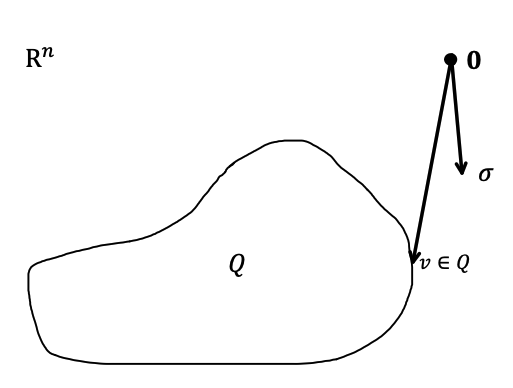
\includegraphics[width=.5\textwidth]{figures/remark2.png}
\end{center}
\caption{We can view empirical Rademacher complexity as the expectation of the maximum inner product between $\sigma$ and $v\in Q$.}
\label{lec6:fig:rs-innerprod}
\end{figure}

Another corollary of this is that the empirical Rademacher complexity doesn't depend on the exact parameterization of $\cF$. For example, suppose we have two parameterizations $\cF = \left\{f(x)=\sum \theta_{i} x_{i} \mid \theta \in \mathbb{R}^{d}\right\}$ and $\cF' = \left\{f(x)=\sum \theta_{i}^{3} \cdot w_{i} x_{i} \mid \theta \in \R^{d}, w \in \mathbb{R}^{d}\right\}$. Since $Q_\cF$ and $Q_{\cF'}$ are the same, we see that $R_S(\cF) = R_S(\cF')$ since our earlier expression for $R_S(\cF)$ only depends on $\cF$ through $Q_\cF$. 

\subsec{Rademacher complexity is translation invariant}
A useful fact is that both empirical Rademacher complexity and average Rademacher complexity are translation invariant. (This is not obvious when thinking of how translation affects the picture in Figure \ref{lec6:fig:rs-innerprod}.)

\begin{proposition}
Let $\cF$ be a family of functions mapping $Z \mapsto \R$ and define $\cF' = \{f'(z) = f(z) + c_0\mid f\in \cF\}$ for some $c_0\in\R$. Then $R_S(\cF) = R_S(\cF')$ and $R_n(\cF) = R_n(\cF')$.
\end{proposition}

\begin{proof}
We will prove here that empirical Rademacher complexity is translation invariant.
\begin{align}
R_S(\cF') &= \E_{\sigma_1,\dots, \sigma_n} \l[ \sup_{f'\in \cF'} \frac{1}{n} \sum^n_{i=1} \sigma_i f(z_i) \r] \\
&= \E_{\sigma_1,\dots, \sigma_n} \l[ \sup_{f\in \cF} \frac{1}{n} \sum^n_{i=1} \sigma_i (f(z_i)+c_0) \r] \\
&= \E_{\sigma_1,\dots, \sigma_n} \l[ \frac{1}{n} \sum^n_{i=1} \sigma_i c_0 + \sup_{f\in \cF} \frac{1}{n} \sum^n_{i=1} \sigma_i f(z_i) \r] \\
&= \E_{\sigma_1,\dots, \sigma_n} \l[\sup_{f\in \cF} \frac{1}{n} \sum^n_{i=1} \sigma_i f(z_i) \r] = R_S(\cF), \label{lec6:eqn:rs-translation}
\end{align}
where \eqref{lec6:eqn:rs-translation} follows because $\E_{\sigma_1,\dots,\sigma_n} \frac{1}{n}\sum_{i=1}^n \sigma_i c_0 = 0$, since the $\sigma_i$'s are Rademacher random variables.
\end{proof}

